%========================================================================================
% Latex-Beamer-Template
% TU Dortmund, Informatik Lehrstuhl VII
%========================================================================================
\documentclass[10pt]{beamer}

\usetheme{tufi}
\usepackage{wasysym}
\usepackage[ngerman]{babel}
\usepackage[utf8]{inputenc}
\usepackage{amsmath,amsfonts,amssymb}
\usepackage{graphicx}
\usepackage[T1]{fontenc}
\usepackage{verbatim}
\usepackage[babel,german=quotes]{csquotes}
\usepackage{array}
\usepackage{multirow}
\usepackage{rotating}
\usepackage{pgfpages}
\usepackage[backend=biber]{biblatex}
\bibliography{Literatur.bib}

\newcommand\tabrotate[1]{\begin{turn}{90}\rlap{#1}\end{turn}}
\newcommand\MyBox[2]{
  \fbox{\lower0.75cm
    \vbox to 1.7cm{\vfil
      \hbox to 1.7cm{\hfil\parbox{1.4cm}{#1\\#2}\hfil}
      \vfil}%
  }%
}

%========================================================================================
% Hier Vortragstitel, Autor und Vortragsdatum eintragen
\pdfinfo
{
  /Title       (Zeit-Effizientes Training von Convolutional Neural Networks)
  /Creator     (TeX)
  /Author      (Jessica Bühler)
}


\title{Masterarbeit -- Zeit-Effizientes Training von Convolutional Neural Networks}
\author{Jessica Bühler}
\date{\today}
%========================================================================================

\begin{document}

\frame{\titlepage}

\AtBeginSection[]
{
  \frame<handout:0>[allowframebreaks]
  {
    \frametitle{Übersicht}
    \tableofcontents[currentsection,hideallsubsections]
  }
}

\AtBeginSubsection[]
{
  \frame<handout:0>[allowframebreaks]
  {
    \frametitle{Übersicht}
    \tableofcontents[sectionstyle=show/hide,subsectionstyle=show/shaded/hide]
  }
}

\newcommand<>{\highlighton}[1]{%
  \alt#2{\structure{#1}}{{#1}}
}

\newcommand{\icon}[1]{\pgfimage[height=1em]{#1}}


%=Inhalt=================================================================================
\section{PruneTrain}
\begin{frame}{}
\begin{figure}
 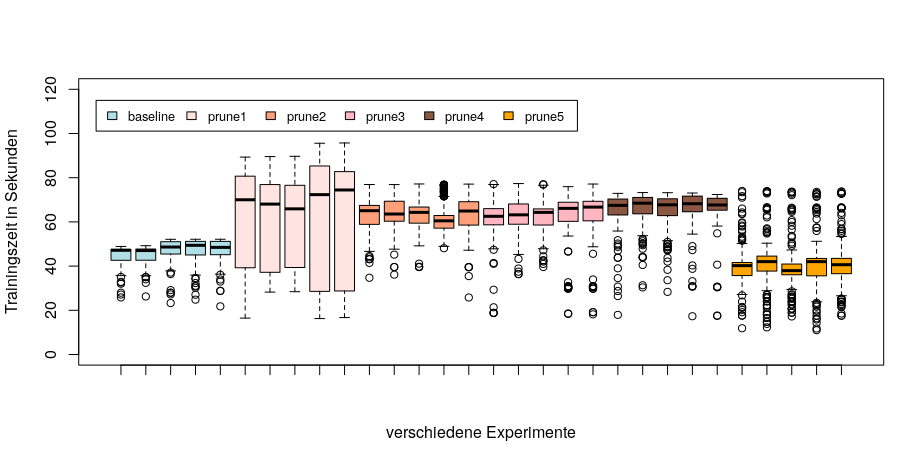
\includegraphics[width=0.7\textwidth]{grafik/prune.png}
 % cnn.jpeg: 1255x424 px, 72dpi, 44.27x14.96 cm, bb=0 0 1255 424
 \caption{Übersicht über die Zeiten}
\end{figure}
prune1-prune4 sind Experimente ohne Anpassung der Batchgröße währenddem Training 

prune5 Anpassung der Batchgrösse währenddem Training
\end{frame}



\begin{frame}{}
 \begin{figure}
 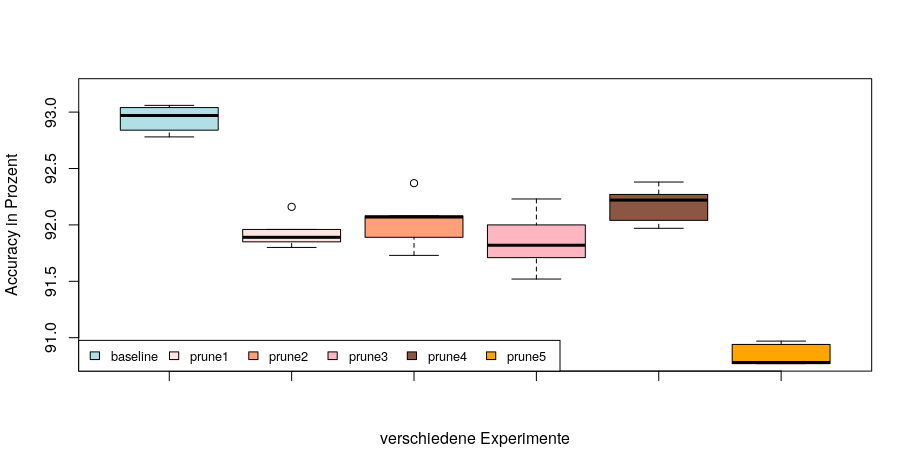
\includegraphics[width=0.9\textwidth]{grafik/pruneVsbaselineAcc.png}
 % module.conv1.weight_12.png: 640x480 px, 100dpi, 16.26x12.19 cm, bb=0 0 461 346
 \caption{Übersicht über die Accuracy}
\end{figure}
Accuracy Verlust durch Prune5 2,6\%
 
\end{frame}

\begin{frame}{}
\begin{itemize}
 \item  Im PruneTrain Paper zeigt sich bereits beim Anwenden von PruneTrain ohne Anpassung der Batch Size ein Verringerung der Trainingszeit
 \item Dieses Ergebnis lässt sich leider nicht reproduzieren. Da dort mehrere GPU parallel benutzt werden, wird hier vorallem an der Kommunikation zwischen den GPU gespart wird. 
 \item Beim Anpassen der Batchsize währenddem Pruning wird hier etwa 12\% Prozent gespart.
 \item Wobei sich hier gezeigt hat, dass neben der Anpassung der Batchgrösse auch wichtig ist dass die richtige Lernrate genutzt wird.
\end{itemize}
\end{frame}


\begin{frame}{}
 \begin{figure}
 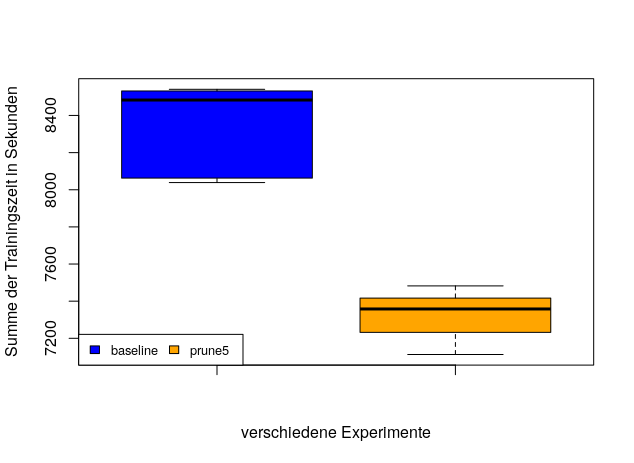
\includegraphics[width=0.9\textwidth]{grafik/pruneVsBaseline.png}
 % module.conv1.weight_12.png: 640x480 px, 100dpi, 16.26x12.19 cm, bb=0 0 461 346
 \caption{}
\end{figure}
\end{frame}

\section{Large Batch}

\begin{frame}{Large Batch}
\begin{itemize}
 \item Large Batch sorgt bei einer grösseren Batchsize (4000 staat 256) dafür, dass weiterhin ein grosser Teil des Netzwerks geprunt werden kann.
 \item Bei Large Batch wird nicht der komplette Speicher genutzt. Hier sind noch weitere Untersuchungen fällig.
 \item bei Cifar10 konnte bei einer grossen Batch size keine Generalization Gap beobachtet werden -> Cifar100 oder ImageNet
\end{itemize}
\end{frame}



\end{document}
